\section{Specific Requirements}
\subsection{External Interface Requirements}
\subsubsection{User Interfaces}
The user interface of eMall is a mobile application, with an easy to use design.
It should be available on every major mobile operating system.
On the other hand, the interface of the CPMS subsystem is a web application with a dashboard with all the available features.
It should be available on every major web browser.
\subsubsection{Hardware Interfaces}
The system is fully operated on the Internet, so it doesn't feature any hardware interface, apart from the device needed to access the service.
%\subsubsection{Software Interfaces}
\subsubsection{Communication Interfaces}
The main communication interfaces of the platform are the users and CPOs.
The system interacts with users to receive booking requests or to send information, and to CPOs to let them select different charging station options.
%%%
\subsection{Functional Requirements}

\subsubsection{Use case diagrams}
\begin{enumerate}
    \item \textbf{Unregistered Customer}
    \begin{figure}[H]
        \begin{center}
            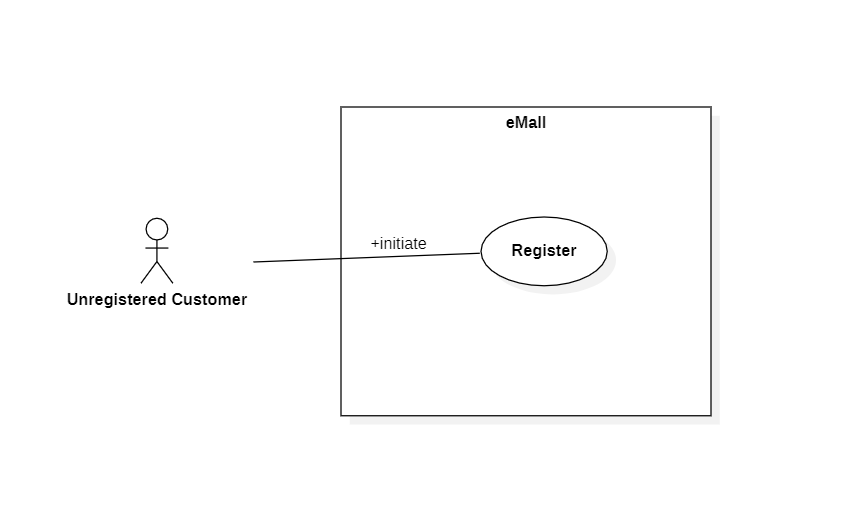
\includegraphics[width=\textwidth]{img/Unregistered_customer.PNG}
            \caption{Unregistered Customer - Use Case Diagram}
        \end{center}
    \end{figure}

    \item \textbf{Registered Customer}
    \begin{figure}[H]
        \begin{center}
            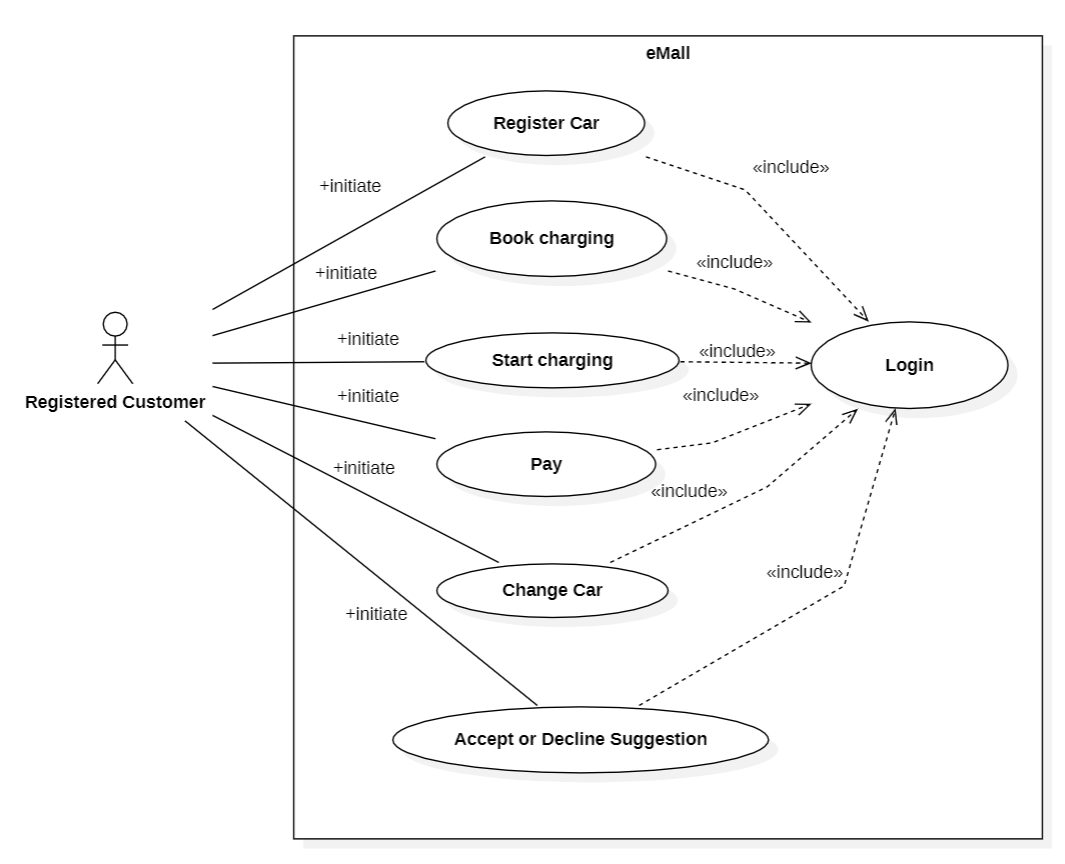
\includegraphics[width=\textwidth]{img/Registered_customer.PNG}
            \caption{Registered Customer - Use Case Diagram}
        \end{center}
    \end{figure}

    \item \textbf{Charging Point Operator}
    \begin{figure}[H]
        \begin{center}
            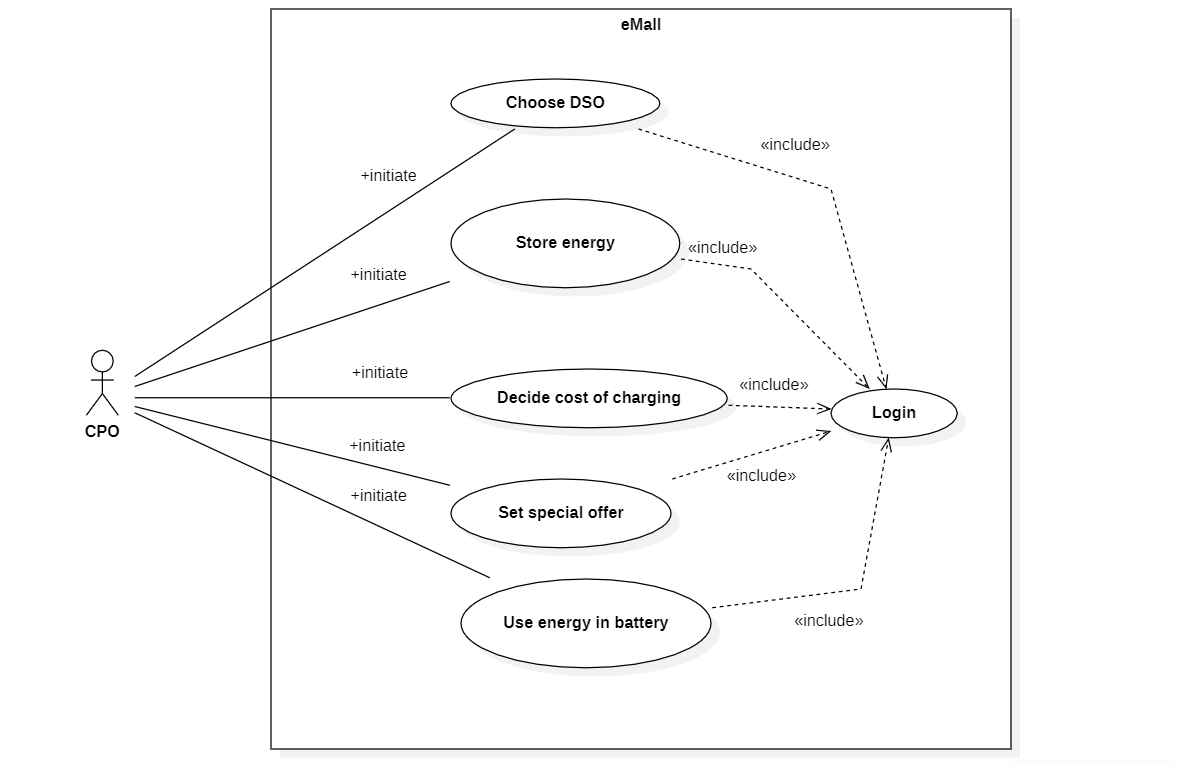
\includegraphics[width=\textwidth]{img/CPO_UseCase.PNG}
            \caption{Charging Point Operator - Use Case Diagram}
        \end{center}
    \end{figure}

\end{enumerate}
\subsubsection{Use case tables}
%%SIGNUP
\begin{longtable}{ | c | p{10cm} | }

    \hline
    ID               & 1                        \\ \hline
    Name             & Sign Up Customer   \\
    \hline
    Actor            & Unregistered Customer \\
    \hline
    Entry conditions &
    \begin{itemize}
        \item Unregistered Customer has downloaded and opened the application on his smartphone
    \end{itemize}
    \\
    \hline

    Input            & \begin{itemize}
        \item username
        \item email
        \item password
        \item birthdate
    \end{itemize} \\ \hline
    Events flow      & \begin{itemize}[nosep,after=\strut]
        \item The application displays the Sign In screen
        \item Unregistered Customer clicks on "Sign Up"
        \item The application displays a list of fields that User must compile: username, email, password, birthdate
        \item Unregistered Customer inserts the mandatory data and accepts the "Terms of Services"
        \item Unregistered Customer clicks on confirm button
        \item The application displays the acceptance of registration and invites the Customer to go on his inbox in order to confirm the registration
        \item Customer opens his inbox, checks the e-mails and clicks on confirmation link
    \end{itemize} \\
    \hline
    Exit conditions  & Customer registration has been successful: user data are stored in the database of the system. Customer can now Login with his credentials. \\ \hline
    Output           & \begin{itemize}
        \item The email of the Customer is stored in the database of the application
        \item The Customer receives the email of confirmation
    \end{itemize} \\
    \hline
    \hline
    Exception 1      & Customer inserts an e-mail which is already stored in the database. So, after he inserts his data and clicks on confirm, the application displays an error page which tells him that he is already registered to the service and invites him to login with that e-mail. \\
    \hline
    Exception 2      & Customer inserts an invalid e-mail. So, after the Customer clicks on the confirm button, the application displays the same page and an error message, which suggests to the Customer to check the e-mail inserted or to change it. \\
    \hline
    \caption{Sign Up Customer} \\
\end{longtable}
%%LOGIN
\begin{longtable}{|c| p{10cm}|}
    \hline ID        & 2 \\
    \hline
    Name             & Login Customer on the application\\
    \hline
    Actor            & Customer \\
    \hline
    Entry conditions & \begin{itemize}[nosep,after=\strut]
        \item Customer has downloaded and opened the application on his smartphone
        \item Customer has registered to the service
    \end{itemize}\\ \hline
    Input            & Customer email and password associated to a valid registration \\
    \hline
    Events flow      & \begin{itemize}[nosep,after=\strut]
        \item The system displays the Login page
        \item Customer inserts in apposite fields the credentials for logging in and presses the Login button.
        \item The system checks the correctness of the credential inserted.
        \item The system displays the home page of the application.
    \end{itemize} \\
    \hline
    Exit condition   & User is logged in \\
    \hline
    \hline
    Exception 1      & Customer inserts a wrong combination of credentials and presses Login button. In this case, the system detects the error and the application displays the Login page with an error. \\
    \hline
    \caption{Login Customer} \\
\end{longtable}
%%BOOK A CHARGE
\begin{longtable}{|c| p{10cm}|}
    \hline ID        & 3\\
    \hline
    Name     & Book a Charge \\
    \hline
    Actor            & Customer\\
    \hline
    Entry conditions & Customer has logged in \\
    \hline
    Events flow      & \begin{itemize}[nosep,after=\strut]
        \item The application displays the home page, which is a map with all the nearby charging stations.
        \item The Customer chooses a charging station.
        \item The application displays all information about a charging station, including its current availability.
        \item The Customer selects an available station and type of socket for the recharge and clicks the confirm button.
        \item The application displays a confirm popup, with the essential details of the upcoming booking.
        \item Customer clicks the confirm button.
    \end{itemize}\\
    \hline
    Exit condition   & The application displays a brief summary of the booking, including the unique ID number of the booking.\\
    \hline
    Output           & \begin{itemize}
        \item   The system has the received the booking, and will mark the socket as booked for 15 minutes, and then either the booking is fulfilled by the Customer, or the system will mark the socket as available.
        \item   The Customer sees the summary in his bookings section, with a reminder that the booking only lasts 15 minutes.
    \end{itemize}\\
    \hline
    \hline
    Exception 1      &  Customer selects an unavailable charging station. In this case, the application displays an error message stating the situation, with the time for the first socket of the selected type to be available. \\
    \hline
    Exception 2      & Customer presses on confirm button, but he has already booked a socket currently. In this case, the application displays an error page, and redirects the Customer to the home page.       \\
    \hline
    \caption{Book a charge}\\
\end{longtable}
%%REMOTELYSTART
\begin{longtable}{|c| p{10cm}|}
    \hline ID        & 4\\
    \hline
    Name     & Remotely Start a Charge \\
    \hline
    Actor            & Customer\\
    \hline
    Entry conditions & \begin{itemize}[nosep,after=\strut]
        \item Customer has booked a charge and has driven his car to the socket of the said booking in time.
        \item Customer has opened the application and logged in.
    \end{itemize}
        \\
    \hline
    Events flow      & \begin{itemize}[nosep,after=\strut]
        \item The application displays a map with all the nearby charging stations.
        \item The Customer selects the "Bookings" menu from the side menu.
        \item The application displays all his current and previous bookings.
        \item The Customer selects the booking related to current station, socket and time.
        \item The application displays the brief summary of his booking, and also an "Unlock Socket" button.
        \item Customer clicks the button, and then the application displays a confirmation message. 
        \item The Customer connects his electric vehicle to the socket.
        \item The application displays an updated version of the summary of the booking with a "Start Charging" button.
        \item The Customer clicks the said button.
    \end{itemize}\\
    \hline
    Exit condition   & The application displays a confirmation message with the estimated time of charge completion, and then redirects the user to the home page.\\
    \hline
    Output           &  The Customer's vehicle recharges.
    \\
    \hline
    \hline
    Exception 1      &  Customer clicks on the "Start Charging" button while his vehicle is not connected. In this case, the application displays an error message that says the there isn't any vehicle to the socket, and redirects the Customer to the current booking view. \\
    \hline
    \caption{Remotely start a charge}\\
\end{longtable}
%% PAY FUNCTION
\begin{longtable}{|c| p{10cm}|}
    \hline ID        & 5\\
    \hline
    Name     & Pay for the Charging Service \\
    \hline
    Actor            & Customer\\
    \hline
    Entry conditions & \begin{itemize}[nosep,after=\strut]
        \item Customer has used the service for a charge.
        \item Customer has opened the application and logged in.
    \end{itemize}
        \\
    \hline
    Events flow      & \begin{itemize}[nosep,after=\strut]
        \item The application displays a map with all the nearby charging stations.
        \item The Customer selects the "Bookings" menu from the side menu.
        \item The application displays all his current and previous bookings.
        \item The Customer selects the booking related to the one that he wants to pay.
        \item The application displays the brief summary of his booking, and also a "Pay" button.
        \item Customer clicks the button, and then the application redirects him to an external payment platform, where he can input his preferred payment method and then pay. 
    \end{itemize}\\
    \hline
    Exit condition   & The Customer will then be returned to the booking summary once the payment has been finished, with a success message.\\
    \hline
    Output           &  The Customer's booking has been paid.
    \\
    \hline
    \hline
    Exception 1      &  Customer inputs an invalid payment method. In this case, the external services closes and the he is returned to the application. The application then displays an error message that says the payment method is invalid. \\
    \hline
    \caption{Pay for the Charging Service}\\
\end{longtable}
%% SUGGESTION FUNCTION
\begin{longtable}{|c| p{10cm}|}
    \hline ID        & 6\\
    \hline
    Name     & View Suggestions \\
    \hline
    Actor            & Customer\\
    \hline
    Entry conditions & \begin{itemize}[nosep,after=\strut]
        \item Customer has logged in.
        \item Customer has received a push notification about the availability of a suggestion.
    \end{itemize}
        \\
    \hline
    Events flow      & \begin{itemize}[nosep,after=\strut]
        \item The application displays a summary of the suggestion with all the information about the booking to make.
        \item The Customer selects the "Accept" option.
    \end{itemize}\\
    \hline
    Exit condition   & The application displays a brief summary of the booking, including the unique ID number of the booking.\\
    \hline
    Output           & \begin{itemize}
        \item   The system has the received the booking, and will mark the socket as booked for 15 minutes, and then either the booking is fulfilled by the Customer, or the system will mark the socket as available.
        \item   The Customer sees the summary in his bookings section, with a reminder that the booking only lasts 15 minutes.
    \end{itemize}
    \\
    \hline
    \hline
    Exception 1      &  Customer logs in after some time since the notification. The system will check if his current position is close enough to the suggestion and if the type of socket of the suggestion is still available at the station.
    If it is not available, the system won't show the suggestion and the user will be directed to the home page.\\
    \hline
    Exception 2      &  The user selects the "Decline" option. The system will cancel the suggestion and redirect the user to the home page.\\
    \hline
    \caption{View Suggestions}\\
\end{longtable}

%%%CPO USECASES

\begin{longtable}{|c| p{10cm}|}
    \hline ID        & 7\\
    \hline
    Name     & CPO Login \\
    \hline
    Actor            & CPO\\
    \hline 
    Entry conditions & CPO has opened the web portal of his CPMS subsystem.
        \\
    \hline
    Input & The CPO credentials associated with a valid registration.
    \\
    \hline
    Events flow      & \begin{itemize}[nosep,after=\strut]
        \item The website displays the Login screen.
        \item The CPO inputs the credentials.
        \item The system checks for the correctness of the credentials.
        \end{itemize} \\
    \hline
    Exit condition   & CPO is logged in.
    \\
    \hline
    Exception 1      & CPO inserts a wrong combination of credentials and presses Login button. In this case, the system detects the error and the application displays the Login page with an error. \\
    \hline
    \caption{CPO Login}\\
\end{longtable}
\subsubsection{Sequence diagrams}
This section shows all sequence diagrams related to the use cases. In all cases we consider that the actor has already logged in, except in the diagrams representing the registration and the login in operations.


\subsubsection{Requirements}
\begin{enumerate}[label=\textbf{-G\arabic*}:]
    \item {Allow customers to obtain information about nearby charging stations
          \begin{itemize}
              \item \textbf{R1:} The system allows customers to view nearby station.
              \item \textbf{R2:} The system allows customer to select a charging station to view its information.
              \item \textbf{D1:} Each customer who wants to use eMall needs to have a mobile device with the most common mobile OSes (e.g. iOS, Android), and also a reliable Internet connection with that device.
              \item \textbf{D4:} The customer's schedule and location is accessible by the platform.
          \end{itemize}
          }
    \item {Allow customers to book a charge for a certain timeframe
          \begin{itemize}
              \item \textbf{R1:} The system allows customers to view nearby station.  
              \item\textbf{R2:} The system allows customers to select a charging station to view its information.
              \item \textbf{R3:} The system shows available socket for each charging station.
              \item \textbf{R4:} The system allows customer to book an available socket in a charging station.
              \item \textbf{D1:} Each customer who wants to use eMall needs to have a mobile device with the most common mobile OSes (e.g. iOS, Android), and also a reliable Internet connection with that device.
              \item \textbf{D4:} The customer's schedule and location is accessible by the platform.
                            
          \end{itemize}
          }
    \item {Allow customers to start the charge and show predicted charging time
          \begin{itemize}
              \item \textbf{R5:} The system allows customers to view personal bookings.
              \item \textbf{R6:} The system allows customers to select a specific booking.
              \item \textbf{R7:} The system allows to start a charge for a booking when the vehicle is connected and ready to charge.
              \item \textbf{R8:} The system shows to the user the predicted charging time when the charge is started.
              \item \textbf{D1:} Each customer who wants to use eMall needs to have a mobile device with the most common mobile OSes (e.g. iOS, Android), and also a reliable Internet connection with that device.
              \item \textbf{D9:} The vehicle start charging only when it is connected to the booked socket.
              \item \textbf{D10:} The socket notifies the CPMS when a vehicle is attached and ready to charge.
              \item \textbf{D15:} All the sockets present in charging stations feature a system that can retrieve the charging level of a car after it has been connected to the socket.
          \end{itemize}
          }
    \item {Allow customers to know when the charging has finished
          \begin{itemize}
              \item \textbf{R9:} The system show the binary charging state (in charge/finished).
              \item \textbf{R10:} The system recommends alternative day/time slots or store/chains to a user.
              \item \textbf{D1:} Each customer who wants to use eMall needs to have a mobile device with the most common mobile OSes (e.g. iOS, Android), and also a reliable Internet connection with that device.
              \item \textbf{D16:} The socket notifies the CPMS when a vehicle has finished to charge.
          \end{itemize}
          }
    \item {Allow customers to pay for the charging service
          \begin{itemize}
              \item \textbf{R5:} The system allows customers to view personal bookings.
              \item \textbf{R6:} The system allows customers to select a specific booking.
              \item \textbf{R11:} The system allows customers to pay a booked charge.
              \item \textbf{D1:} Each customer who wants to use eMall needs to have a mobile device with the most common mobile OSes (e.g. iOS, Android), and also a reliable Internet connection with that device.
              \item \textbf{D8:} A fully functioning payment system is present and returns if a transaction has been successful or not.
              
          \end{itemize}
          }
    
          \item {Allow customers to receive suggestions on where to charge
          \begin{itemize}
              \item \textbf{R12:} The system periodically searches possible nearby station to charge based on the customer car's battery SoC (<50\%), customer's location, customer's calendar.
              \item \textbf{R13:} The system sends a push notification if a possible nearby station is found and no suggestions were sent in the previous 1h.
              \item \textbf{D1:} Each customer who wants to use eMall needs to have a mobile device with the most common mobile OSes (e.g. iOS, Android), and also a reliable Internet connection with that device.
              \item \textbf{D3:} The customer's mobile device fully supports the push notification technology.
              \item \textbf{D4:} The customer's schedule and location is accessible by the platform.
              \item \textbf{D6:} The data automatically obtained by the system in order to send suggestions to the customer is accurate and truthful.
              \item \textbf{D14:} Given a license plate number and personal identification, it exists an API that provides the battery level of the vehicle associated with the license plate.
              
          \end{itemize}
          }


          \item {Allow Charging Point Operators to decide the energy acquisition options
          \begin{itemize}
              \item \textbf{R:} 
              \item \textbf{R:} 
              \item \textbf{R:} 
              \item \textbf{R:} 
              \item \textbf{D2:} Each CPO who wants to access the CPMS platform needs to have a device connected to the Internet (such as PC, Mac, smartphone, etc), with the most common Web Browsers (e.g. Firefox, Google Chrome, Microsoft Edge, Apple Safari, etc).
              \item \textbf{D11:}Every CPO is supplied with login credentials when the system is installed.
              \item \textbf{D8:}
              \item \textbf{D8:} 
              
          \end{itemize}
          }


          \item {Allow Charging Point Operators to dynamically choose the charging cost and to set offers
          \begin{itemize}
              \item \textbf{R:} 
              \item \textbf{R:} 
              \item \textbf{R:} 
              \item \textbf{R:} 
              \item \textbf{D2:} Each CPO who wants to access the CPMS platform needs to have a device connected to the Internet (such as PC, Mac, smartphone, etc), with the most common Web Browsers (e.g. Firefox, Google Chrome, Microsoft Edge, Apple Safari, etc).
              \item \textbf{D11:} Every CPO is supplied with login credentials when the system is installed.
              \item \textbf{D8:}
              \item \textbf{D8:}
              \item \textbf{D8:} 
              
          \end{itemize}
          }
\end{enumerate}

\subsubsection{Traceability Matrix}
%TODO mapping between requirements and use cases
\subsection{Performance Requirements}

Performance requirements are not particularly critical for the system, but it is anyway desirable that the system has a good response time, which could be included between 0.1 and 2 seconds.
Otherwise, Customers and CPOs may think that the service is interrupted or does not work.
Moreover the system has to guarantee a good experience for all users, taking into account that not everyone has access to high speed internet. Therefore,
the system should minimize the amount of broadband needed in order to fully
download the content.
The server infrastructure will be designed to be scalable so that it will be possible to adapt it to
the increment of users when the application diffusion will increase.
Finally, the system should be able to handle many concurrent users, at least
100 000.
\subsection{Design Constraints}
\subsubsection{Standards Compliance}

The system must be compliant to the GDPR law, as it will mainly used in EU. \newline
Secure connections must be used for data comunicaction. \newline
Customers must accept and read the privacy policy during the sign-up phase. \newline

\subsubsection{Hardware Limitations}

Each customer is required to have a smartphone device on which it is possible to install the eMall application. The device must have access to the internet. \newline
The CPO must have access to the internet using a web browser on a PC.  



\subsection{Software System Attributes}

\begin{enumerate}[label=\textbf{NFR\arabic*}:]
    \item \textbf{Reliability}\\
    The system must prevent downtime, in order to let Customers to charge their vehicle in every moment. At the same time CPO must be granted to access the system and perform their actions all the time.
    To guarantee that the system is up most of the time, preventive regular maintanance should be perfomed. To make the system 24/07 accesible the server could be duplicated and the duplicated one run in parallel. So that during failures and maintanance, of one of them, users can access the other one. 
    \item \textbf{Availability}\\
    Given the fact that eMall is not an emergency service or anything related to critical situations, the system must provide availability of 99.9\%. This means that the average time between the occurrence of a fault and service recovery (MTTR) has to be contained at around 0.365 days per year.
    \item \textbf{Security}\\
    The data provided by the users contain some sensitive information, so the security aspect cannot be underestimated. The central database must be protected with all the available measures to avoid any external or internal attack. The passwords inside the data store have to be encrypted and in case of password recovery, this must never be sent in clear.
    Communication between parties are encrypted and goes on a secure channel (through SSL protocol) to avoid traffic sniffing and spoofing, thus avoiding cheating attacks and guaranteeing privacy and consistency.
    \item \textbf{Maintainability}\\
    The system must guarantee a high level of maintainability. It must be designed in such a way that permits future addition of functionalities with minimum effort.
    Design techniques must in fact guarantee an high reusability. The code must be well documented and hard-coding must be avoided. A testing routine has to be provided and it has to cover at least 75\% of the entire codebase, excluding interfaces code.
    \item \textbf{Portability}\\
    The application must be developed for two different platforms: iOS and Android smartphones. The web application must run on any OS (like Windows, Mac OS, Linux, etc) that supports a web browser. Even mobile devices like iPads and Android tablets must be able to access the web app.
\end{enumerate}

